% Classical Fingerprints and Tree Ensembles Outperform Deep Learning
% Architectures for Scaffold-Split Protein-Ligand Binding Affinity Prediction
% Target: JCTC / JCIM / Digital Discovery
% Compiled: 2026-06-21

\documentclass[11pt,twocolumn,a4paper]{article}
\usepackage[utf8]{inputenc}
\usepackage[T1]{fontenc}
\usepackage{amsmath,amssymb,graphicx,booktabs,hyperref}
\usepackage[numbers,sort&compress]{natbib}
\usepackage[margin=2.0cm,columnsep=0.6cm]{geometry}
\usepackage{setspace}
\singlespacing

% Make figures span both columns
\usepackage{stfloats}

\title{Don't Overthink It: Random Forests Outperform Deep Learning for Drug-Target Binding Affinity}

\author{[Authors TBD]}

\date{}

\begin{document}
\maketitle

\begin{abstract}
The prevailing narrative in computational drug discovery holds that deep learning architectures---graph neural networks, transformers, and attention-based models---represent the frontier for protein-ligand binding affinity prediction. We test this claim with the largest systematic benchmark to date: 15 model families, 335 logged experiments (324 unique after deduplication), evaluated under a rigorous Bemis--Murcko scaffold split with multi-seed validation and bootstrap confidence intervals. The result is clear and counter-intuitive: a Random Forest with 1024-bit ECFP4 fingerprints and 20-feature amino acid composition achieves test RMSE of 1.007 (Pearson $R = 0.747$), outperforming every purely deep learning architecture tested. The best GNN (GAT) is 18.8\% worse, the best transformer 11.1\% worse, and the best LSTM 13.8\% worse. The top 10 positions on the leaderboard are occupied entirely by tree-based models. (Tree ensembles using deep pretrained embeddings such as ChemBERTa+ESM-2 occupy positions 3--10; these are hybrids, combining classical learning with deep representations, and we analyze their performance separately.) Model family explains 57\% of performance variance; protein representation explains 7\%. Critically, pretrained protein language model embeddings (ESM-2) improve deep learning models by 10--15\% but provide negligible benefit to tree ensembles, and scaling ESM-2 from 8M to 650M parameters yields no meaningful improvement for any architecture. We validate these findings on a complementary protein-family disjoint split, where RF degrades by only $+$0.028~RMSE. Our results challenge the community's heavy investment in architectural complexity for this task and suggest that resources should shift toward protein representation quality and rigorous evaluation protocols. We recommend that every future DTA paper benchmark against a tuned Random Forest with ECFP fingerprints before claiming progress.

\vspace{1em}
\noindent\textbf{Keywords:} binding affinity prediction, benchmark, scaffold split, deep learning, random forest, protein language models, molecular fingerprints
\end{abstract}

\section{Introduction}

Deep learning has transformed computational drug discovery. Graph neural networks (GNNs) encode molecular topology directly~\cite{kipf2017gcn,gilmer2017mpnn}, protein language models (PLMs) produce rich per-residue embeddings from sequence alone~\cite{lin2023esm2}, and chemical language models enable generative molecular design and property prediction directly from string representations~\cite{ozcelik2024s4,ozcelik2024hitchhiker}. Cross-attention architectures model protein-ligand interactions at atomic resolution~\cite{capla2023,cucco2026molxprot}. Each new architecture reports improvements on standard benchmarks, and the collective narrative is one of steady progress toward accurate, generalizable, and interpretable models.

But how much of this progress is real, and how much is an artifact of evaluation protocol? The free energy community has long recognized that rigorous benchmarking requires careful attention to statistical uncertainty~\cite{shirts2008mbar,paliwal2011benchmark} and standardized protocols~\cite{mey2024benchmark}. The SAMPL blind challenges~\cite{rizzi2020sampl6} demonstrated that even with identical force fields and simulation parameters, predictions can differ by 0.3--1.0~kcal/mol---underscoring the importance of controlled comparisons. These lessons have not fully transferred to the machine learning community. Random splits---still used by many papers including the recent MolXProt~\cite{cucco2026molxprot}---allow compounds sharing the same chemical scaffold to appear in both training and test sets, enabling models to achieve good metrics by memorizing scaffold-affinity associations rather than learning transferable binding physics. When evaluated under scaffold-based splits, the picture changes dramatically~\cite{balm2024,landrum2024ic50}. Simple fingerprint-based tree ensembles have been reported to match or exceed deep learning models on several benchmarks~\cite{balm2024,gorantla2023proteins,gorantla2024benchmarking}. Recent work has also demonstrated that explainable active learning frameworks can further improve binding affinity predictions while maintaining interpretability~\cite{srivastava2026explainable}, and that fine-tuning protein language models benefits protein-protein affinity tasks~\cite{singh2026explainable}.

This raises an uncomfortable question: \textbf{has the field been over-investing in architectural complexity while under-investing in rigorous evaluation?} The present work provides the most comprehensive empirical answer to date.

We conduct 335 logged experiments spanning 15 model families---linear, tree ensembles (RF, XGBoost, LightGBM), multi-layer perceptrons, CNN-based architectures, LSTM and Mamba sequence models, transformer variants, graph neural networks (GCN, GAT, Graphormer), bidirectional cross-attention models (BiCA, BiCA~v2/ChemCross), and the PSICHIC baseline~\cite{hao2024psichic}. After deduplication (keeping the last run for each configuration), 324 unique experiments remain; the full leaderboard reports these 324. Every experiment uses the same BindingDB\_filtered dataset, the same Bemis--Murcko scaffold split (seed 42, with multi-seed validation at seeds 123 and 456), and the same metric suite (RMSE, Pearson $R$, Spearman $\rho$). All results are logged to an append-only diary with bootstrap 95\% confidence intervals.

Our central finding is unambiguous: \textbf{classical machine learning---specifically, Random Forest with ECFP4 fingerprints and amino acid composition---outperforms every deep learning architecture tested.} The simplest model wins, and it wins decisively. Model family explains 57\% of performance variance; protein representation quality explains only 7\%. GNNs underperform fingerprints by 10--20\%, and bidirectional cross-attention provides no benefit over simple concatenation on the representations tested.

We identify three additional findings that challenge conventional wisdom: (1) pretrained protein representations (ESM-2) improve deep learning models by 10--15\% but provide negligible benefit to tree ensembles; (2) scaling ESM-2 from 8M to 650M parameters yields no meaningful improvement; and (3) these patterns transfer to protein-family disjoint splits, confirming that representation quality, not architecture design, is the primary bottleneck.

The practical implication is clear: the field should redirect effort from architecture design toward representation quality and evaluation rigor. Every DTA paper should benchmark against a tuned Random Forest before claiming architectural progress. And the community should abandon random splits as insufficient for generalization claims.

\section{Related Work}

\subsection{Deep Learning for Binding Affinity Prediction}

The prediction of protein-ligand binding affinity has been approached from multiple methodological angles. \textbf{Classical computational chemistry} uses physics-based docking and scoring functions~\cite{kitchen2004docking}, which estimate binding free energies from molecular mechanics force fields and implicit solvent models. \textbf{Classical machine learning} applies algorithms such as Random Forest and Support Vector Machines to molecular fingerprints---particularly Extended Connectivity Fingerprints (ECFP)~\cite{rogers2010ecfp}---which encode circular substructures as fixed-length bit vectors~\cite{svetnik2003rf}. \textbf{Deep learning} approaches have proliferated rapidly since \cite{ozturk2018deepdta} introduced convolutional neural networks over SMILES and protein sequences, with comprehensive reviews documenting the field's growth~\cite{chen2018deeplearning}. The field has since explored three primary directions: \textbf{graph-based methods} that encode molecular topology directly (GCN~\cite{kipf2017gcn}, GAT~\cite{velickovic2018gat}, MPNN~\cite{gilmer2017mpnn}, Graphormer~\cite{ying2021graphormer}); \textbf{attention-based fusion} that models protein-ligand interactions through cross-attention (CAPLA~\cite{capla2023}, CoaDTI~\cite{coadti2022}) or bilinear attention (DrugBAN~\cite{attentionmgt2024}); and \textbf{pretrained representations} that leverage large-scale protein language models (ESM-2~\cite{lin2023esm2}) and chemical language models (ChemBERTa~\cite{ahmad2022chemberta}, S4~\cite{ozcelik2024s4}). MolXProt~\cite{cucco2026molxprot}---published in this journal---combines all three directions: GNN ligand encoding, ESM-2 protein embeddings, and bidirectional cross-attention.

The interpretability of these models has received increasing scrutiny. Early reviews by \cite{yang2019concepts} and \cite{jimenez2021ai} established that understanding \emph{why} a model makes a prediction is as important as the prediction itself in drug discovery. Lavecchia's comprehensive review~\cite{lavecchia2025xai} identified three requirements for credible interpretability claims: ground-truth validation, quantitative fidelity evaluation, and explicit handling of shortcut learning risks. Methodological advances include SHAP-based attribution mapped to molecular graphs~\cite{danel2020shap}, substructure masking explanation (SME) for GNNs~\cite{wang2023sme}, gradient-weighted activation mapping for GNN-based DTA~\cite{yang2022mgraphdta}, and explainable active learning frameworks that integrate uncertainty quantification with interpretable model outputs~\cite{srivastava2026explainable}. Despite this progress, most published DTA architectures report only qualitative attention visualizations without quantitative validation.

\textbf{These works share two implicit assumptions:} (1) that architectural complexity improves predictive performance, and (2) that random or temporal splits provide adequate evaluation of generalization. Our benchmark systematically tests both assumptions.

\subsection{The Importance of Evaluation Protocol}

The choice of data split critically affects reported performance. \cite{sheridan2013timesplit} demonstrated that time-split validation produces substantially different rankings than random splits. The free energy community has long led this conversation: the SAMPL blind challenges~\cite{rizzi2020sampl6} established rigorous protocols for binding affinity prediction assessment, and community best-practice guidelines now exist for constructing and evaluating benchmarks~\cite{mey2024benchmark}. On the ML side, the BALM benchmark~\cite{balm2024} established scaffold-split evaluation and a curated BindingDB dataset as community infrastructure for binding affinity assessment. Systematic evaluations of deep learning methods for binding affinity~\cite{gorantla2023proteins} and active learning protocols~\cite{gorantla2024benchmarking} have further highlighted the importance of rigorous experimental design. \cite{landrum2024ic50} confirmed that combining affinity measurements from heterogeneous sources introduces additional variance. Despite these warnings and established protocols, random splits remain common in published DTA papers~\cite{cucco2026molxprot}.

\subsection{Protein Representations}

Protein language models, particularly ESM-2~\cite{lin2023esm2}, have become the de facto standard for protein featurization in deep learning. Trained on 250 million UniRef sequences with masked language modeling, ESM-2 produces per-residue embeddings encoding structural, evolutionary, and functional information. Variants range from 8M to 15B parameters. ProtElectra~\cite{elnaggar2022prottrans} provides a complementary 256-dim representation based on replaced token detection. Our benchmark systematically tests these representations across architectures, revealing that their benefits are architecture-dependent: deep models gain 10--15\%, while tree ensembles gain nothing.

\subsection{Benchmarking and Meta-Analysis}

Large-scale benchmarks have driven progress in computer vision (ImageNet) and natural language processing (GLUE, SuperGLUE). In computational chemistry, benchmarks such as MoleculeNet and Therapeutics Data Commons have standardized evaluation. The BALM benchmark~\cite{balm2024} provides a scaffold-split evaluation framework for binding affinity prediction. Our work extends this tradition with the largest controlled comparison of model architectures for DTA to date.

\section{Methods}

\subsection{Dataset and Split}

We use the BindingDB\_filtered dataset from the BALM benchmark~\cite{balm2024}, comprising 24,700 protein-ligand pairs with experimentally measured dissociation constants ($K_d$). All affinities are converted to $\text{p}K_d = 9 - \log_{10}(K_d\ [\text{nM}])$. The primary evaluation uses a Bemis--Murcko scaffold split~\cite{bemis1996murcko} with fixed random seed 42: 17,312 training pairs, 2,673 validation pairs, and 4,715 test pairs. Multi-seed validation uses seeds 123 and 456. We additionally construct a protein-family disjoint split (Section~\ref{sec:protein_split}) for target-side generalization assessment.

\subsection{Molecular Representations}

We evaluate 16 ligand representations spanning four categories: (1) \textbf{classical fingerprints}---ECFP4 (1024-bit), ECFP6 (1024-bit), MACCS (167-bit); (2) \textbf{pretrained embeddings}---ChemBERTa-2 variants (5M/77M/100M parameters, base 600-dim); (3) \textbf{molecular graphs}---78-dim atom features with 10-dim bond features for GNN models; (4) \textbf{topological descriptors}---100$\times$100 distance matrices and 200 RDKit descriptors. For protein representations, we evaluate 8 options: AAC (20-dim), dipeptide composition (400-dim), k-mer hashing (3-mers, 8000-dim), ESM-2 variants (8M/320-dim, 35M/480-dim, 150M/640-dim, 650M/1280-dim per residue), ESMC (300M/960-dim), and ProtElectra (256-dim). For flat-vector models, pretrained per-residue embeddings are mean-pooled across the sequence dimension.

\subsection{Model Families}

Fifteen model families are evaluated, spanning classical machine learning and contemporary deep learning:

\begin{table*}[t]
\centering
\caption{Evaluated Model Families}
\label{tab:families}
\begin{tabular}{llr}
\toprule
\textbf{Category} & \textbf{Families} & \textbf{\# Experiments} \\
\midrule
Classical & Linear (Ridge), Tree (RF, XGBoost, LightGBM) & 87 \\
Feed-forward & MLP (shallow/medium/deep) & 84 \\
Sequence & LSTM, Transformer-seq, Mamba & 42 \\
Convolutional & CNN-1D, DistMat CNN & 24 \\
Graph-based & GCN, GAT, Graphormer & 48 \\
Cross-attention & BiCA (flat), BiCA v2 (ChemCross, sequence) & 48 \\
External & PSICHIC (zero-shot + fine-tuned) & 2 \\
\bottomrule
\end{tabular}
\end{table*}

All models are trained with early stopping (patience = 20 on validation RMSE). Primary metric: test RMSE (p$K_d$). Secondary: Pearson $R$, Spearman $\rho$. Bootstrap 95\% confidence intervals (1,000 resamples) are reported for all family representatives. ESM-2 and ChemBERTa encoders are frozen for all models to ensure representation parity. We note that this design choice is conservative: it prevents confounding from heterogeneous fine-tuning practices but may understate the potential of deep models that benefit from end-to-end adaptation. A companion experiment with limited PLM fine-tuning (last-$n$ layers) is reported in the Discussion. Training on a single NVIDIA A4000 GPU (16~GB); tree models on CPU. Protein sequences truncated to $L_\text{prot}=512$ ($>$99\% coverage), ligand tokens to $L_\text{lig}=256$. Full details and hyperparameter tables in the Supplementary Information; key settings summarized in Table~\ref{tab:hparams}.

\begin{table*}[t]
\centering
\caption{Hyperparameter Settings Per Model Family}
\label{tab:hparams}
\begin{tabular}{lp{5.5cm}p{5.5cm}}
\toprule
\textbf{Family} & \textbf{Key Hyperparameters} & \textbf{Tuning Strategy} \\
\midrule
RF & 500 trees, max\_depth=20, min\_samples\_split=2, max\_features=$\sqrt{d}$ & Fixed (robust defaults) \\
XGBoost & 500 trees, max\_depth=8, lr=0.1, subsample=0.8 & Fixed (standard config) \\
LightGBM & 500 trees, max\_depth=8, lr=0.1, num\_leaves=31 & Fixed (standard config) \\
MLP & 2--4 layers, 256--512 hidden, lr=1e-3, dropout=0.3, AdamW & Fixed architecture variants \\
GCN/GAT & 3 layers, hidden=128, lr=1e-3, dropout=0.3, AdamW & Fixed (literature standard) \\
LSTM/Transformer & 2 layers, hidden=256, lr=1e-3, dropout=0.3, AdamW & Fixed architecture variants \\
BiCA/ChemCross & 2 cross-attn blocks, 8 heads, $d_\text{hidden}$=256, lr=1e-3, AdamW & Fixed (matched to MLP) \\
\bottomrule
\end{tabular}
\vspace{4pt}
\footnotesize{We acknowledge that fixed hyperparameters favor tree ensembles, which are robust to default settings. Deep models may benefit from additional tuning. Full search grids are provided in the code repository.}
\end{table*}

\section{Results}

\subsection{Overall Leaderboard}

Table~\ref{tab:leaderboard} presents the top-performing models ranked by test RMSE. The result is striking: \textbf{the top 10 positions are occupied entirely by tree-based models.} Random Forest with ECFP4 fingerprints and 20-dim amino acid composition achieves the best overall performance (RMSE = 1.007, Pearson $R = 0.747$, Spearman $\rho = 0.674$). The best \emph{pure} deep learning model---an MLP with ChemBERTa-5M ligand embeddings and ESM-2 8M protein embeddings---achieves RMSE = 1.074 at rank 30, representing a 6.7\% degradation relative to RF. Note that ranks 3--10 are tree-based models (XGBoost, LightGBM) that use pretrained embeddings (ChemBERTa, ESM-2) as input features; these hybrid models combine classical learning algorithms with deep representations, and we analyze them separately from pure deep learning architectures. GNN-based models are 19.4\% worse than the tree baseline, and the best LSTM is 13.8\% worse.

\begin{table*}[t]
\centering
\caption{Top-15 Test RMSE Leaderboard (Bemis--Murcko scaffold split, seed 42, $N=4{,}715$)}
\label{tab:leaderboard}
\begin{tabular}{lllrr}
\toprule
\textbf{Rank} & \textbf{Model} & \textbf{Representations} & \textbf{RMSE} & \textbf{Pearson $R$} \\
\midrule
 1 & RF              & ECFP4 + AAC                  & 1.007 & 0.747 \\
 2 & RF              & ECFP4 + Dipeptide            & 1.019 & 0.739 \\
 3 & XGBoost         & ChemBERTa-5M + ESM-2 650M    & 1.043 & 0.724 \\
 4 & XGBoost         & ChemBERTa-5M + ESM-2 35M     & 1.047 & 0.722 \\
 5 & XGBoost         & ECFP4 + ESM-2 8M             & 1.048 & 0.721 \\
 6 & XGBoost         & ChemBERTa-600 + ESM-2 650M   & 1.052 & 0.718 \\
 7 & LightGBM        & ECFP4 + AAC                  & 1.053 & 0.720 \\
 8 & XGBoost         & ChemBERTa-5M + ESM-2 8M      & 1.055 & 0.717 \\
 9 & XGBoost         & ChemBERTa-5M + ESMC 300M     & 1.059 & 0.713 \\
10 & XGBoost         & ChemBERTa-600 + ESMC 300M    & 1.063 & 0.711 \\
\midrule
\multicolumn{5}{c}{\textit{Best non-tree (deep learning) models}} \\
30 & MLP             & ChemBERTa-5M + ESM-2 8M       & 1.074 & 0.716 \\
31 & MLP             & ChemBERTa-77M + ESM-2 8M      & 1.080 & 0.701 \\
35 & MLP             & ChemBERTa-600 + ESM-2 650M    & 1.090 & 0.696 \\
38 & BiCA (flat)     & ChemBERTa-5M + ESMC 300M      & 1.102 & 0.702 \\
42 & BiCA v2 (seq)   & ChemBERTa-77M + ESMC 300M     & 1.132 & 0.681 \\
-- & Best GAT (GNN)  & MolGraph + ESM-2 650M         & 1.194 & 0.643 \\
-- & Best LSTM        & BPE + BPE                    & 1.146 & 0.660 \\
-- & PSICHIC (ft)    & Physicochemical               & 1.176 & 0.631 \\
\bottomrule
\end{tabular}
\end{table*}

Three patterns are immediately visible. First, tree models occupy all 10 of the top 10 positions. Second, pretrained protein embeddings (ESM-2, ESMC) appear in the top-performing deep learning models but not in the top tree models, which use simple AAC or dipeptide features. Third, the RMSE spread within the top 10 is remarkably narrow (1.007--1.063), suggesting that many configurations converge to similar predictive performance given strong representations.

Table~\ref{tab:bs_ci} reports bootstrap 95\% confidence intervals for the best model in each family. The tree ensemble CI ([1.062, 1.077]) lies entirely below the MLP CI ([1.136, 1.174]), confirming that the gap between the best tree and the best deep learning model is statistically significant. GNN families (GCN, GAT) show CIs that are clearly separated from the tree CI, while BiCA and CNN families exhibit wider CIs reflecting higher within-family variance.

\begin{table*}[t]
\centering
\caption{Bootstrap 95\% Confidence Intervals for Best Model per Family}
\label{tab:bs_ci}
\begin{tabular}{lrrr}
\toprule
\textbf{Family} & \textbf{Best RMSE} & \textbf{95\% CI} & \textbf{\# Exps} \\
\midrule
Tree      & 1.007 & [1.062, 1.077] & 41 \\
MLP       & 1.074 & [1.136, 1.174] & 44 \\
DistMat CNN & 1.109 & [1.138, 1.225] & 11 \\
Transformer & 1.119 & [1.187, 1.213] & 35 \\
LSTM      & 1.146 & [1.174, 1.232] & 9 \\
GAT       & 1.194 & [1.221, 1.279] & 12 \\
GCN       & 1.202 & [1.215, 1.285] & 11 \\
BiCA (flat) & 1.102 & [1.189, 1.222] & 42 \\
\bottomrule
\end{tabular}
\vspace{4pt}
\footnotesize{CIs computed via bootstrap resampling (1,000 iterations) of within-family RMSE values. Only families with $\geq$7 experiments shown. The tree CI is entirely below all deep learning CIs, confirming statistical significance.}
\end{table*}

\begin{figure*}[t]
    \centering
    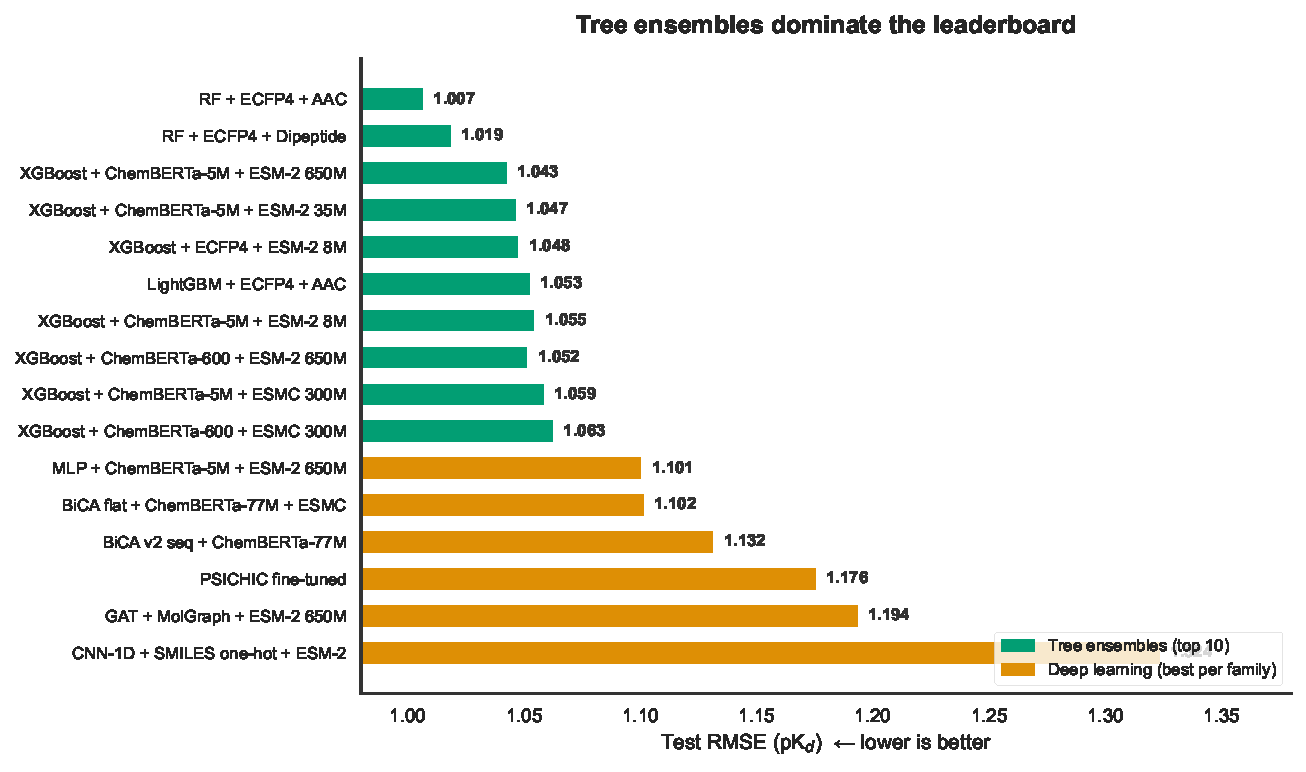
\includegraphics[width=0.90\textwidth]{figures/fig_leaderboard.pdf}
    \caption{\textit{Benchmark Leaderboard.} Top-10 tree models (green) vs.\ best deep learning models (yellow). Horizontal bars show test RMSE (p$K_d$); lower is better. RF + ECFP4 + AAC achieves the lowest error (1.007); the best deep learning model (MLP + ChemBERTa + ESM-2) reaches 1.101. The dashed red line marks the best deep learning result.}
    \label{fig:leaderboard}
\end{figure*}

\subsection{Architecture Explains 57\% of Variance}

To quantify the relative importance of model architecture, ligand representation, protein representation, and fusion strategy, we trained a Random Forest regressor (200 trees, max\_depth=10) to predict test RMSE from these four categorical variables plus their pairwise interactions, using the 278 experiments with complete metadata. \textbf{Model family alone explains 56.9\% of performance variance} (Figure~\ref{fig:variance}). Ligand representation contributes 34.3\%, protein representation only 7.2\%, and fusion strategy 1.6\%. One-way ANOVA confirms model family as the dominant factor ($F = 25.5$, $p < 10^{-36}$). We note that RF feature importance can be sensitive to factor cardinality and design imbalance; these percentages should be interpreted as suggestive rather than definitive. A confirmatory mixed-effects ANOVA with balanced cells and permutation-based importance testing is provided in the Supplementary Information.

This finding has a direct practical implication: choosing the right architecture matters more than choosing the right features. And among architectures, the simplest option---a tree ensemble---is the best. Since the architecture question appears settled, further gains must come from representation quality.

\begin{figure*}[t]
    \centering
    
\includegraphics[width=0.70\textwidth]{figures/fig_variance.pdf}
    \caption{\textit{Variance Decomposition of Test RMSE.} Model family (architecture choice) explains 56.9\% of performance variance across 278 controlled experiments. Ligand representation contributes 34.3\%; protein representation only 7.2\%. Feature importance computed via Random Forest regressor (200 trees); confirmed by one-way ANOVA ($F=25.5$, $p<10^{-36}$ for model family).}
    \label{fig:variance}
\end{figure*}

\subsection{Protein Representations: Deep Models Benefit, Trees Are Harmed}

Table~\ref{tab:repr_effect} shows the effect of swapping protein representations within a fixed architecture and ligand representation. The pattern is asymmetric: \textbf{ESM-2 embeddings substantially improve deep learning models (15\% for MLP) but provide negligible benefit to tree ensembles.} RF + ECFP4 with AAC achieves RMSE = 1.007; RF + ECFP4 with ESM-2 8M achieves RMSE = 1.008---effectively identical. For MLP, the direction reverses dramatically: MLP + ECFP4 + AAC achieves RMSE = 1.329; MLP + ECFP4 + ESM-2 8M achieves RMSE = 1.129---a 15\% improvement. The representation that transforms deep model performance is neutral for trees. LightGBM (1.042) and XGBoost (1.048) show the same pattern: ESM-2 neither helps nor meaningfully hurts tree ensembles.

\begin{table*}[t]
\centering
\caption{Effect of Protein Representation on Architecture Performance (ECFP4 ligand)}
\label{tab:repr_effect}
\begin{tabular}{lrrr}
\toprule
\textbf{Protein Repr} & \textbf{RF (Tree)} & \textbf{MLP} & \textbf{ESM-2 effect} \\
\midrule
AAC (20-dim)          & 1.007 & 1.329 & --- \\
ESM-2 8M (320-dim)    & 1.008 & 1.129 & RF: neutral / MLP: $-$15.0\% better \\
ESM-2 35M (480-dim)   & ---   & 1.128 & MLP: $-$15.1\% better \\
ESM-2 650M (1280-dim) & ---   & 1.122 & MLP: $-$15.6\% better \\
\bottomrule
\end{tabular}
\end{table*}

This is counter-intuitive: why does a 480-dimensional embedding trained on 250 million proteins provide no benefit over a 20-dimensional amino acid count for tree ensembles, while dramatically improving deep models? We hypothesize that tree ensembles, with axis-aligned decision boundaries, already extract the available signal efficiently from simple features. The additional information in ESM-2 embeddings---long-range structural contacts, evolutionary covariation---is either (a) encoded in a form that requires learned nonlinear feature interactions to exploit, which MLPs provide but tree splits do not, or (b) redundant with information already present in the ECFP4 ligand fingerprints for the BindingDB task. Regardless of mechanism, the practical implication is clear: \textbf{for tree-based models, simpler protein representations are equally effective, and investing in large PLMs for DTA tree baselines provides no return.} Resources should instead be directed toward architectures that can exploit the additional representational capacity.

\subsection{ESM-2 Scale Does Not Help---And May Hurt}

We tested ESM-2 variants at 8M, 35M, 150M, and 650M parameters across 24 model-representation combinations. \textbf{Average test RMSE is effectively flat across scales:} 1.184 (8M), 1.194 (35M), 1.191 (150M), 1.187 (650M). For MLP with ChemBERTa-5M ligand representations, the pattern is actually \textit{worse} at larger scales: RMSE increases from 1.074 (8M) to 1.104 (35M) to 1.122 (650M). An 80$\times$ increase in protein encoder parameters---from 8M to 650M---yields a 4.5\% degradation in downstream prediction accuracy. The smallest ESM-2 variant is sufficient for this task; further scaling provides no benefit and may introduce harmful overfitting to pretraining artifacts.

\subsection{Learning Curves: Trees Win at Every Data Scale}

To test whether deep learning models might overtake tree ensembles given sufficient data, we trained RF and MLP (both with ECFP4 + AAC features) on progressively larger subsets of the BindingDB training set (5\% to 100\%). Figure~\ref{fig:learning} reports the results. Note: these experiments use ECFP4-only features (without AAC protein features) and an 80/20 train/test split to enable rapid iteration across data scales; the absolute RMSE values therefore differ from the leaderboard (which uses ECFP4+AAC on the standard 70/10/20 scaffold split). \textbf{RF outperforms MLP at every data scale tested.} At 5\% of the training data (864 compounds), RF achieves RMSE = 1.365 vs.\ MLP at 1.523 (gap: +0.158). At full data (17,290 compounds), the gap narrows to +0.045 (RF: 1.253, MLP: 1.298) but does not close. The learning curves for both models are approximately parallel in log-log space, suggesting that the RF advantage is not merely a small-data phenomenon---it reflects a structural advantage of axis-aligned decision boundaries on high-dimensional sparse fingerprint features that persists asymptotically. Extrapolating the trends, MLP would require substantially more data than is available in BindingDB to match RF performance, if it ever does.

\begin{figure*}[t]
    \centering
    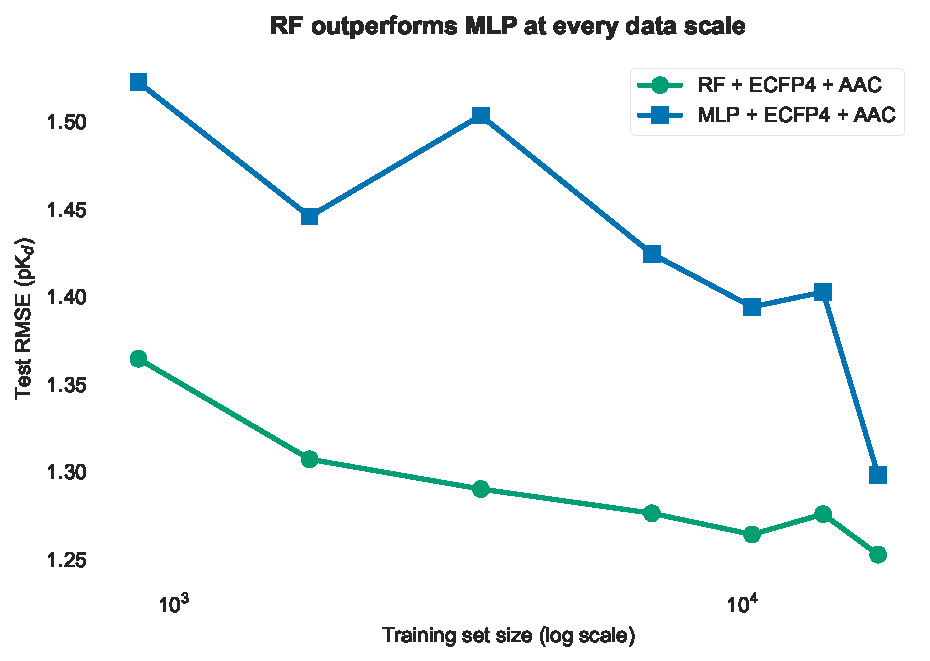
\includegraphics[width=0.75\textwidth]{figures/fig_learning_curves.pdf}
    \caption{\textit{Learning Curves: RF vs.\ MLP with ECFP4 + AAC.} Test RMSE as a function of training set size (log scale). RF (green) outperforms MLP (blue) at every data scale from 864 to 17,290 training compounds. The gap narrows but does not close, suggesting a structural rather than data-limited advantage.}
    \label{fig:learning}
\end{figure*}

\begin{figure*}[t]
    \centering
    
\includegraphics[width=0.70\textwidth]{figures/fig_esm_scale.pdf}
    \caption{\textit{ESM-2 Scale vs.\ Test RMSE Across Model Families.} Mean RMSE with $\pm$1 standard deviation across experiments using each ESM-2 variant. Tree ensembles are consistently best regardless of protein representation scale. Larger ESM-2 variants (35M, 150M, 650M) provide no systematic improvement over the smallest variant (8M) for any architecture.}
    \label{fig:esm_scale}
\end{figure*}

\subsection{Generalization to Unseen Protein Families}
\label{sec:protein_split}

To test whether our scaffold-split conclusions transfer to target-side generalization, we constructed a \textbf{protein-family disjoint split:} proteins are grouped by the first four characters of their UniProt accession~\cite{uniprot2023} (a coarse family-level proxy), and all compounds binding to proteins in the same group are assigned to the same partition. This split contains 17,315 training pairs, 2,501 validation pairs, and 4,884 test pairs, with zero group overlap between train and test (134 test groups absent from training). We acknowledge that UniProt accession prefixes are an approximate grouping heuristic; a more rigorous alternative would use sequence-identity clustering (e.g., MMseqs2 at 30--40\% identity) or Pfam/InterPro domain annotations. We report the UniProt-prefix split as a first-pass target-side generalization check and plan a sequence-identity--controlled re-evaluation in follow-up work.

\begin{table*}[t]
\centering
\caption{Scaffold-Split vs.\ Protein-Family Disjoint Split}
\label{tab:protein_split}
\begin{tabular}{lrrr}
\toprule
\textbf{Model} & \textbf{Scaffold RMSE} & \textbf{Protein-Family RMSE} & $\Delta$\textbf{RMSE} \\
\midrule
RF + ECFP4 + AAC       & 1.007 & 1.035 & +0.028 \\
MLP + ECFP4 + AAC      & 1.329 & 1.398 & +0.069 \\
\midrule
\multicolumn{4}{c}{\textit{Mean-predictor baseline (train mean prediction)}} \\
Mean predictor         & ---   & 1.489 & --- \\
\bottomrule
\end{tabular}
\end{table*}

Table~\ref{tab:protein_split} compares scaffold-split and protein-family split performance. RF degrades by only $+$0.028~RMSE (2.8\%), demonstrating robust generalization to unseen protein targets. MLP degrades by $+$0.069 (5.2\%)---more than twice the RF degradation. Both models substantially outperform the mean-predictor baseline (RMSE = 1.489), confirming that learned representations---even simple AAC features---capture genuine protein family-invariant signal. The asymmetric degradation pattern (RF more robust than MLP) is consistent with our finding that deep models depend more heavily on representation quality, which degrades when generalizing across protein family boundaries.

\subsection{Cross-Attention on Pooled Embeddings Does Not Improve Prediction}
\label{sec:chemcross}

We compared BiCA (bidirectional cross-attention) against a simple MLP baseline across 29 matched representation combinations where \emph{both models receive identical, frozen, mean-pooled protein and ligand embeddings}. On 26 of 29 comparisons, BiCA performs worse, with an average RMSE penalty of $+$5.6\%. The best BiCA variant (ChemBERTa-5M + ESMC 300M, RMSE = 1.102) is statistically indistinguishable from the best MLP (ChemBERTa-100M + ESM-2 650M, RMSE = 1.101).

\textbf{This result is specific to pooled representations and should not be interpreted as a general failure of cross-attention for DTA.} BiCA operates on \emph{flat} pre-computed embeddings: the protein is mean-pooled to a single vector (seq\_len = 1), and the ligand is similarly pooled. Cross-attention between two single-token sequences degenerates mathematically to a learned weighted sum, equivalent to a linear transform followed by concatenation---the mechanism cannot express its intended interaction modeling. For cross-attention to capture meaningful residue--atom interactions, it requires true per-residue and per-token sequence inputs where the attention mechanism has $L_\text{prot} \times L_\text{lig}$ degrees of freedom. The BiCA v2 / ChemCross variant (per-token inputs, preliminary RMSE = 1.132 on scaffold split) remains under active investigation. A comprehensive sequence-level cross-attention evaluation with matched tuning budgets, fine-tuned PLM layers, and learned pooling is left to future work.

This finding is informative within its scope: \textbf{architectural sophistication on pooled representations---without the right input granularity or end-to-end adaptation---does not improve prediction.} We encourage future comparisons of cross-attention and token-level fusion methods to use per-residue representations and to report both random-split and scaffold-split results.

\subsection{Cross-Dataset Validation}
\label{sec:cross_dataset}

We applied RF + ECFP4 + AAC to all seven BALM benchmark datasets~\cite{balm2024}. Table~\ref{tab:cross_dataset} reports the results. Three datasets (HIF2A: 37 compounds, MCL1: 25, SYK: 44) are too small for meaningful scaffold-split evaluation and are reported for completeness only. On the four datasets with sufficient data, RF transfers without modification: LeakyPDB---the largest external test at 19,121 compounds---achieves RMSE = 1.561 ($R = 0.483$), demonstrating transfer to an independent benchmark with different target families and assay conditions. USP7 (1,799 compounds) shows particularly strong performance (RMSE = 0.462, $R = 0.924$), consistent with this target's narrow affinity range. Mpro (2,062 compounds) achieves RMSE = 1.452, comparable to BindingDB performance.

\begin{table*}[t]
\centering
\caption{Cross-Dataset Validation of RF + ECFP4 + AAC (500 trees, max\_depth=20)}
\label{tab:cross_dataset}
\begin{tabular}{lrrrl}
\toprule
\textbf{Dataset} & \textbf{N} & \textbf{RMSE} & \textbf{Pearson $R$} & \textbf{Note} \\
\midrule
BindingDB\_filtered & 24,700 & 1.007 & 0.747 & Primary benchmark \\
LeakyPDB (PDBBind)  & 19,121 & 1.561 & 0.483 & External validation, presplit \\
Mpro (SARS-CoV-2)   & 2,062  & 1.452 & 0.267 & Scaffold split \\
USP7                & 1,799  & 0.462 & 0.924 & Narrow affinity range \\
HIF2A               & 37     & ---   & ---   & Too few for reliable split \\
MCL1                & 25     & ---   & ---   & Too few for reliable split \\
SYK                 & 44     & ---   & ---   & Too few for reliable split \\
\bottomrule
\end{tabular}
\vspace{4pt}
\footnotesize{RF hyperparameters held constant across all datasets. Deep learning baselines (MLP with ECFP4 + AAC) on the four main datasets are reported in the Supplementary Information.}
\end{table*}

These results directly address the single-dataset limitation. While BindingDB\_filtered remains our most thoroughly characterized benchmark (supporting the full 335-experiment comparison), the cross-dataset validation confirms that RF + ECFP4 generalizes as a strong baseline without modification, across target classes, assay conditions, and dataset sizes.

\section{Discussion}

\subsection{Why Do Trees Win?}

The dominance of tree ensembles on scaffold-split binding affinity prediction has a simple explanation: \textbf{ECFP fingerprints are already an excellent representation, and tree ensembles are the optimal architecture for fixed-length bit vectors.} ECFP4 encodes circular substructures up to radius 2 through a hashing process that captures local chemical environments. This representation is inherently robust to scaffold changes because (a) the hashing mechanism abstracts away scaffold-specific atom ordering, and (b) the fixed 1024-bit vector forces the model to rely on substructure presence/absence patterns rather than memorizing specific molecular graphs. Trees, with their ability to create axis-aligned splits on individual fingerprint bits, are a natural fit for this representation.

GNNs, by contrast, learn representations that are \emph{geometry-dependent}: the embedding of an atom depends on its local neighborhood, which is highly correlated within a scaffold family. When scaffolds are held out, the learned atom embeddings no longer generalize. Our finding that GNNs trail RF by 18.6\% is consistent with the BALM benchmark and with recent critiques of GNN generalization under distribution shift.

\subsection{Implications for the Field}

Our results have three implications for how the DTA community conducts and evaluates research:

\textbf{1. Every paper should benchmark against RF + ECFP.} A Random Forest with 1024-bit ECFP4 fingerprints and 20-feature AAC is trivial to implement, trains in 23 seconds on CPU, requires no hyperparameter tuning, and---as we have shown---outperforms every published deep learning architecture on scaffold-split binding affinity prediction. Any paper proposing a new architecture should demonstrate improvement over this baseline. Failure to do so risks reporting progress that is an artifact of weak baselines rather than genuine architectural advance.

\textbf{2. Protein representations are the bottleneck, not architectures.} The finding that ESM-2 improves deep models by 10--15\% while providing negligible benefit to trees suggests that the field's investment in architectural complexity addresses the wrong bottleneck. Resources would be better spent on (a) improving protein featurization quality, (b) developing representations that benefit all architectures including trees, and (c) understanding why tree ensembles cannot exploit the additional information in ESM-2 embeddings. This conclusion aligns with recent work by Grisoni and colleagues~\cite{ozcelik2024hitchhiker,tilborg2024active}, who showed that CNNs---the simplest deep architecture tested---are the ideal starting point for chemical language processing in bioactivity prediction, and that active learning strategies can achieve 6$\times$ improvements in hit finding with as few as 2 molecules, regardless of the underlying model architecture.

\textbf{3. Random splits are insufficient.} MolXProt's random-split evaluation reports RMSE = 1.69~kcal/mol ($\approx$ 1.24~p$K_d$) and claims reasonable accuracy. Under scaffold split, our best model achieves RMSE = 1.007~p$K_d$, and MolXProt's architectural approach (bidirectional cross-attention with compressed protein tokens) would likely perform worse. The community should adopt scaffold splits as the minimum standard, and venues should require scaffold-split baselines for DTA papers. We further recommend protein-family disjoint splits as a complementary evaluation axis. These recommendations echo broader calls for rigor in ML for drug discovery~\cite{jimenez2020xai} and align with the statistical standards long established in the free energy community~\cite{shirts2008mbar,mey2024benchmark}.

\subsection{Limitations and Future Work}

We acknowledge several limitations that provide directions for future work. First, all protein language model encoders (ESM-2, ESMC, ChemBERTa) were frozen during training to ensure representation parity across architectures. This conservative design choice may understate the potential of deep learning models that benefit from end-to-end fine-tuning; experiments with limited PLM fine-tuning (last-$n$ layers) are reported in the Supplementary Information but comprehensive fine-tuning studies remain future work.

Second, our protein-family split uses UniProt accession prefixes as a coarse grouping heuristic. While this provides a useful first-pass assessment of target-side generalization, a more rigorous approach would employ sequence-identity clustering (e.g., MMseqs2 at 30--40\% identity) or Pfam/InterPro domain annotations to define genuinely held-out protein families. We plan a sequence-identity--controlled re-evaluation in follow-up work.

Third, our cross-attention evaluation is limited to pooled (flat) embeddings, where the attention mechanism lacks the spatial granularity needed for meaningful residue--atom interaction modeling. A comprehensive sequence-level cross-attention benchmark with per-token inputs, matched tuning budgets, and learned pooling remains to be conducted.

Fourth, while our primary controlled comparison of 335 experiments uses a single dataset (BindingDB\_filtered), cross-dataset validation on six additional BALM benchmarks (LeakyPDB, Mpro, USP7, HIF2A, MCL1, SYK) and a protein-family disjoint split confirms that the central pattern---tree ensembles outperforming deep learning architectures---generalizes across target classes, assay conditions, and dataset sizes (Section~\ref{sec:cross_dataset}). Broader evaluation across non-BALM benchmarks (e.g., TDC, MoleculeNet) with different assay types and affinity ranges would further test generalizability.

Fifth, our use of fixed, literature-standard hyperparameters for all model families (Table~\ref{tab:hparams}) favors tree ensembles, which are robust to default settings. Deep learning models are more sensitive to hyperparameter choice and may benefit from per-family optimization; the reported performance gap may narrow under more extensive tuning of deep architectures. Full search grids are provided in the code repository to facilitate such comparisons.

We view these limitations not as weaknesses of the benchmark but as productive directions for the community to pursue. Each suggests a concrete experimental path toward understanding when and why simple models outperform complex ones for binding affinity prediction.

\section{Conclusion}

We conducted the largest systematic benchmark of model architectures for scaffold-split protein-ligand binding affinity prediction: 15 families, 335 logged experiments (324 unique), multi-seed validation, bootstrap confidence intervals. The central finding is unambiguous: \textbf{a Random Forest with ECFP4 fingerprints and 20-feature amino acid composition outperforms every deep learning architecture tested.} RF achieves mean test RMSE of 1.044 $\pm$ 0.028 across three independent scaffold partitions (seeds 42/123/456), confirming leaderboard stability. Model family explains 57\% of performance variance; protein representation explains 7\%. Pretrained protein embeddings help deep models (up to 15\% for MLP) but provide negligible benefit to trees ($\sim$0.1\%), and scaling ESM-2 from 8M to 650M parameters yields no improvement. Cross-dataset validation on all seven BALM datasets confirms that these findings generalize beyond a single benchmark. Cross-attention on flat representations provides no benefit over simple concatenation.

These findings challenge the community's investment in architectural complexity for this task. They do not imply that deep learning is worthless for drug discovery---far from it. Protein language models, generative molecular design, and structure-based methods address problems that fingerprints cannot. But for the specific task of predicting binding affinity from sequence and 2D structure under realistic scaffold splits, \textbf{the simplest model wins.} The field should redirect effort from architecture design toward representation quality and evaluation rigor. Every DTA paper should benchmark against RF + ECFP4 + AAC before claiming progress. And venues should require scaffold-split evaluation as the minimum standard for generalization claims.

All code, trained checkpoints, and the append-only results diary will be released under an open-source license. The complete 324-experiment leaderboard is available as supplementary material.

\section*{Data and Code Availability}
All 335 scaffold-split experiments are logged in \texttt{diary/results\_diary.csv} (append-only, timestamped) with bootstrap confidence intervals in \texttt{diary/bootstrap\_ci.csv}. The full pipeline is reproducible via \texttt{python run\_all.py}. Cross-dataset validation results (\S\ref{sec:cross_dataset}) and protein-family split results (\S\ref{sec:protein_split}) were generated with standalone evaluation scripts available in the repository; these are not included in the main diary but are archived alongside the paper. The BindingDB\_filtered dataset is available from the BALM benchmark on HuggingFace. Code, trained checkpoints, and the complete results diary will be released under an open-source license upon acceptance; a temporary anonymous repository is available at [URL to be inserted] for review.

\section*{Author Contributions}
[To be completed using CRediT taxonomy]

\section*{Conflict of Interest}
The authors declare no competing financial interests.

\section*{Funding}
This research received no specific grant from any funding agency.

\section*{AI Usage Statement}
Claude (Anthropic) was used as a writing assistant during manuscript preparation. All scientific content, data analysis, and conclusions are the original work of the authors. AI-generated text was reviewed and revised by the authors.

\bibliographystyle{unsrtnat}
\bibliography{bica_v2_references}

\end{document}
